\documentclass[answers]{exam}

% \documentclass[addpoints]{exam}

\usepackage{xeCJK}
\usepackage[utf8]{inputenc}
\usepackage{graphicx}
\usepackage{hyperref}
\usepackage{amsmath}
\usepackage{booktabs}
\usepackage{wrapfig}
\usepackage{color}


\pagestyle{headandfoot}
\firstpageheadrule
\firstpageheader{\textbf{Okayama University}}{\textbf{WANG JING}}{\textbf{素粒子・宇宙基礎論}}
\runningheader{Okayama University}
{}
{素粒子・宇宙基礎論}
\runningheadrule
\firstpagefooter{}{Page \quad\thepage\ }{}
\runningfooter{}{Page\quad\thepage\ }{}
%\allowdisplaybreaks


% no box for solutions
% \unframedsolutions

\setlength\linefillheight{.5in}

\renewcommand{\solutiontitle}{\noindent\textbf{Answer:}}
% \renewcommand{\solutiontitle}{\noindent\textbf{解:}\par\noindent}

\renewcommand{\questionlabel}{\thequestion .}
\renewcommand{\thepartno}{\arabic{partno}}
\renewcommand{\partlabel}{\thepartno .}


\begin{document}
\vspace{5mm}
\begin{questions}
\question Solve the Friedman equation in the matter-dominant flat universe and show the time dependence of the scale factor. Show the distance $d$ to a celestial body having the red shift of $z$ is given in the equation below, considering the light ray equation of $ds^{2} = −c^{2}dt^{2}+a^{2}dr^{2} = 0$:
\begin{align*}
d=\frac{2 c}{H_{0}}\left(1-\frac{1}{\sqrt{1+z}}\right)
\end{align*}
Show the Hubble's law when  $z \ll 1$ . Calculate the size of the observable universe in light year
in the limit of $ z \rightarrow \infty$ .
\begin{solution}
The Friedman equation is:
\begin{align}
\left(\frac{\dot{a} }{a}\right)^{2}&=\frac{8 \pi G}{3 c^{2}} \rho
\end{align}
Where $\rho = \rho^{r}+\rho^{m}+\rho^{de}$, consider the matter-dominant period:
\begin{align}
\left(\frac{\dot{a} }{a}\right)^{2} &=\frac{8 \pi G}{3 c^{2}} \rho^{m}=\frac{8 \pi G}{3 c^{2}} \cdot \frac{ \Omega_{m}\rho_{c r}}{a^{3}} \notag \\
&=H_{0}^{2} \Omega_{m} \frac{1}{a^{3}} \notag\\
\sqrt{a}  \dot{a} &=H_{0} \sqrt{\Omega_{m}} 
\end{align}
Integrating both sides,we get
\begin{align*}
\frac{2}{3} a^{\frac{3}{2}} &=H_{0} \sqrt{\Omega_{m}}t\\ 
i.e.\\a(t) &=\left(\frac{3}{2} H_{0} \sqrt{\Omega_{m}} t\right)^{\frac{2}{3}} \\
&\approx\left(\frac{3}{2} H_{0} t\right)^{\frac{2}{3}}    
\end{align*}
Acoording to $c^{2}dt^{2}=a^{2}dr^{2} $, we take squreroot on both sides:
\begin{align}
\frac{dr}{dt}=\frac{c}{a}
\end{align}
In order to get Distance-Redshift relation, we integrating (3) by time :
\begin{align*}
d &= \int_{0}^{t} \frac{c}{a} dt\\
&=\int_{a_{t}}^{a_{t_{0}}} \frac{c}{a}da\cdot\frac{dt}{da}\\
&=\int_{a_{t}}^{a_{t_{0}}} \frac{c}{a\dot{a}}da
\end{align*}
Recall (2) with $\Omega_{m}=1$, we find
\begin{align*}
\dot{a} = H_{0}a^{-\frac{1}{2}}
\end{align*}
Put it in to the integral,
\begin{align*}
d &=\int_{a_{t}}^{a_{t_{0}}} \frac{c}{a\dot{a}}da\\
&=\frac{c}{H_{0}}\int_{a_{t}}^{a_{t_{0}}} a^{-\frac{1}{2}}da\\
&=\frac{2c}{H_{0}}\quad[a^{\frac{1}{2}}]_{a_{t}}^{a_{t_{0}}}
\end{align*}
Recall that $a_{t_{0}} = 1$ and $a_{t}=\frac{1}{1+z}$, so
\begin{align}
d=\frac{2 c}{H_{0}}\left(1-\frac{1}{\sqrt{1+z}}\right)
\end{align}
When $z \ll 1$, we use taylor expansion for (4)
\begin{align*}
d&=\frac{2 c}{H_{0}}\left(1-\frac{1}{\sqrt{1+z}}\right)=\frac{2 c}{H_{0}}\left[1-(1-\frac{1}{2}z)\right]\\
&=\frac{cz}{H_{0}}\\    
\end{align*}
$z$ is Redshift, at low speed approximation
\begin{align*}
\quad z&=\frac{\lambda-\lambda_{0}}{\lambda_{0}}=\frac{\lambda_{0}\left(1+\frac{v}{c}\right)-\lambda_{0}}{\lambda_{0}}=\frac{v}{c}
\end{align*}
So d becomes
\begin{align*}
d&=\frac{v}{H_{0}}\\  
i.e.\\
v&={H_{0}}d\qquad Hubble's\quad Law
\end{align*}
When $ z \rightarrow \infty$, $d=\frac{2 c}{H_{0}}$, and $H_{0}=7.1\times10^{-11}/year$, so the radius of observable universe is $\approx2.82\times10^{10}$ light year.
\end{solution}
\question Show that the photon gas energy density $\rho$ and its pressure P are related with $P = \rho/3$. Given photon’s momentum of p and energy E, show $P = p^2/3E$.
\begin{solution}
The number density of particle in a unit volume, with momenta between p and p + dp is given as
\begin{align*}
n(p) d p=\frac{2}{e^{E_{p}/ k T} - 1} \frac{4 \pi p^{2}}{(2\pi \hbar )^{3}} d p
\end{align*}
Energy density may be calculated as
\begin{align}
\rho = \int_{0}^{\infty}E_{p}n(p) d p
\end{align}
For a given absolute value of velocity and momentum we may calculate the dot-product of the two vectors, and average it over all angles:
\begin{align*}
\mathbf{v p}=v p=v_{x} p_{x}+v_{y} p_{y}+v_{z} p_{z} \\
\left\langle v_{x} p_{x}\right\rangle=\left\langle v_{y} p_{y}\right\rangle=\left\langle v_{z} p_{z}\right\rangle=\frac{1}{3} v p    
\end{align*}
Pressure is defined as a flux of momentum across a unit surface, integrated over all particles.
For an isotropic gas we may select the unit surface to be perpendicular to the ”x” axis, and we may
calculate pressure as
\begin{align}
P=\int_{0}^{\infty}<v_{x} p_{x}>n(p) d p=\frac{1}{3} \int_{0}^{\infty} v(p) p n(p) d p
\end{align}
Especially for photon gas, $v = c, E_{p} = pc$, compare (5) and (6), we can find $P = \rho/3$.\vspace{5mm}\\
\textbf{The equation} $P=\frac{p^{2}}{3E}$ makes no sense (it connects a thermodynamic variables P, to the momentum 
and energy of a single particle). It is also not dimensionally correct. With c=1 momentum p and energy E have the same units, but pressure has units of energy/volume (=energy*momentum3).
\end{solution}







\question  Calculate the number of CMB photons colliding an area of 1 $cm^{2}$ per second.
\begin{solution}
Recall that the enerygy flux of a certain frequency $\nu$ on an unit area per second is:
\begin{align*}
F_{v} &=\int_{2 \pi} \rho_{\gamma}(\nu ) \cdot c \cdot \cos \theta d \Omega\qquad [\rho\quad is\quad energy\quad density] \\
&=\rho_{\gamma}(\nu ) \cdot c \int_{0}^{2 \pi} d \phi \int_{0}^{\frac{\pi}{2}} d \theta \cos \theta \sin \theta \\
&=\rho_{\gamma}(\nu) \cdot c \cdot 2 \pi \int_{0}^{\frac{\pi}{2}} d \theta \frac{1}{2} \sin 2 \theta \\
&=\rho_{\gamma}(\nu ) \cdot c \cdot 2 \pi\cdot  \frac{1}{2}\left[\frac{1}{2}(-1) \cos 2 \theta\right]_{0}^{\frac{\pi}{2}} \\
&=\rho _{\gamma}(\nu) \cdot c \cdot 2 \pi \cdot \frac{1}{2}\left[\frac{1}{2}-\frac{1}{2}(-1)\right]\\
&=\pi \cdot c \cdot \rho_{\gamma}(\nu) \\ 
&=\frac{4 \pi^{2} \hbar}{c^{2}} \frac{\nu ^{3}}{e^{2 \pi \hbar\nu  / k_{B} T}-1}\qquad \left[J / m^{2} / s / H z\right]    
\end{align*}    
So the number of photons of this frequency is:
\begin{align}
N_{\nu}=\frac{F_{\nu}}{\hbar\nu}&=\frac{4 \pi^{2}}{c^{2}} \frac{\nu ^{2}}{e^{2 \pi \hbar\nu/ k_{B} T}-1}
\end{align} 
Integrat (7) over all frequency, we got N, the number of CMB photons colliding an area of 1 $cm^{2}$ per second
\begin{align*}
Set\quad \frac{2 \pi \hbar v}{k_{B} T}=x \quad  \quad \nu &=\frac{k_{B} T}{2 \pi \hbar} x \quad d \nu =\frac{k_{B} T}{2 \pi \hbar} d x\\
N&=\frac{k_{B}^{2}T^{2} }{c^2\hbar ^2} \int _{0} ^{\infty}\frac{x^{2}}{e^{x}-1} d x
\end{align*}
According to Riemann zeta function, $\zeta(3) \Gamma(3)=1.202\times 2=2.404$, and insert the CMB temperature $T=2.73K$ so
\begin{align*}
N&=\frac{[8.62\times 10^{-5}]^2\times 2.73^2\times 2.404}{200^2} \frac{eV^2\cdot K^{-2}\cdot K^{2}}{nm^2\cdot eV^2}\\ 
&=3.328\times10^{-12}/nm^{2}\approx333/cm^{2}
\end{align*}
\end{solution}

\question  Explain why the cross section of the Thomson scattering of a proton is much smaller than that of an electron. Calculate the ratio of the cross sections of a proton to an electron.
\begin{solution}
The differential cross section of Thomson scattering is 
\begin{align*}
\frac{d \sigma}{d \Omega}=\left(\frac{q^{2}}{4 \pi \varepsilon_{0} m c^{2}}\right)^{2} \frac{1+\cos ^{2} \theta}{2}
\end{align*}
And total cross section is 
\begin{align}
\sigma=\frac{8 \pi}{3}\left(\frac{q^{2}}{4 \pi \varepsilon_{0} m c^{2}}\right)^{2}   
\end{align}
According to (8), we can see the cross section has square inverse relation with mass of the scattering particle, this explain why cross section of a proton is much smaller than that of an electron.
And we can estimate the ratio of the cross section of a proton to an electron:
\begin{align*}
\frac{\sigma_{p}}{\sigma_{e}} = \frac{m_{e}^{2}}{m_{p}^{2}}=\frac{0.511^{2}}{938.272^{2}}=2.97\times 10^{-7}
\end{align*}
\end{solution}







\question Explain the origin of the CMB polarization.
\begin{solution}
The CMB polarization originates from rescattering of the primordial photons on the hot electron gas on their way to us.
A quadrupole anisotropy of the photon flux at one point on the last scattering surface generates a polarization in the direction of observation.  
The cross-section of Thomson scattering is s proportional to the square of the scalar product of the incoming and outgoing photons polarizations:
\begin{align*}
\frac{d \sigma}{d \Omega}=\frac{3}{8 \pi}\left|\hat{\varepsilon}^{\prime} \cdot \hat{\varepsilon}\right|^{2} \sigma_{T}   
\end{align*}
Thus outgoing photons only carry polarization orthogonal to the scattering
plane as shown in Figure 1. Radiation fluxes from different directions are incoherent, therefore intensities from opposite incident directions add up,
and only even multipoles of the flux angular distribution contribute. 
\end{solution}
\begin{figure}[h]
\centering
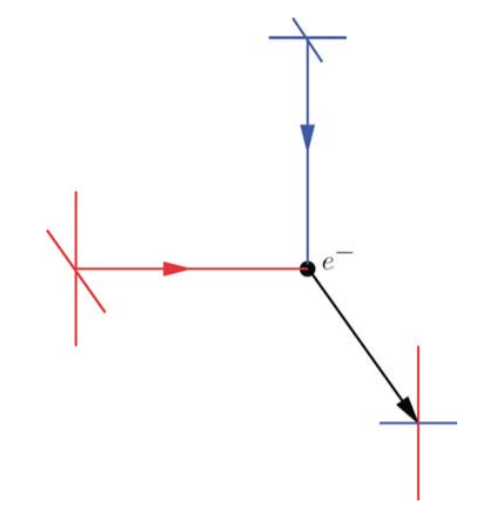
\includegraphics[width=8cm]{Figure/7.png}
\caption{ Polarization from Thomson scattering.}
\end{figure}

\begin{figure}[h]
\centering
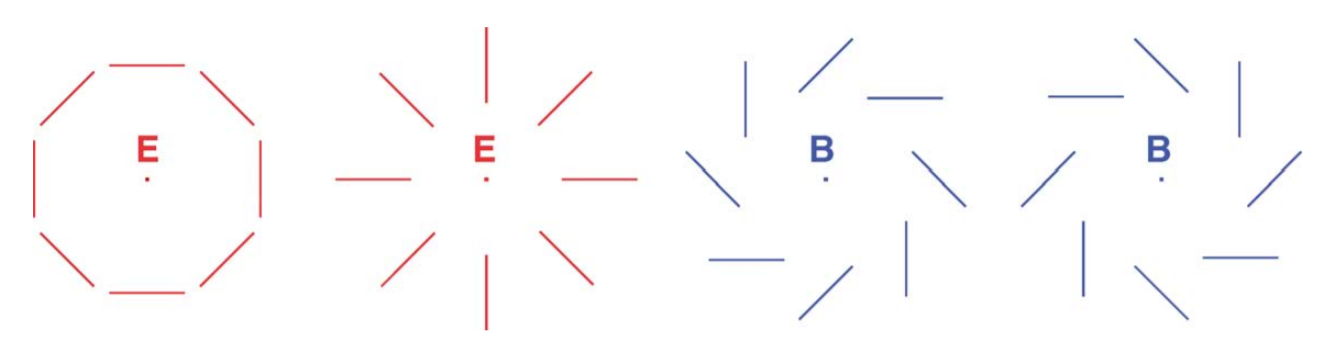
\includegraphics[width=13cm]{Figure/8.png}
\caption{  Typical E or B type polarization patterns.}
\end{figure}






\end{questions}

\end{document}